% =====================================================================
%  INTERNSHIP REPORT — Full Stack Development of KioMeet
%  Student: Aman Verma (23bcs012)  |  Company: IndiWebPros
%  Compiled with XeLaTeX (uses system Palatino font).
%  Formatting per SMVDU internship-report template:
%    - A4, Top=2.54cm, Bottom=2.54cm, Left=3.0cm, Right=2.0cm
%    - Font: Palatino, 12pt body, 1.5 line spacing, justified
%    - Title 24pt regular; candidate name 14pt regular
%    - Chapter headings: 14pt bold, uppercase
%    - Heading 1 (section): 12pt bold, uppercase
%    - Heading 2 (subsection): 12pt bold, title case
%    - Heading 3 (subsubsection): 12pt italic, title case
%    - Preliminary pages numbered in lowercase roman; Chapter 1 onward in arabic
% =====================================================================
\documentclass[12pt,oneside,a4paper]{report}

\usepackage[a4paper,top=2.54cm,bottom=2.54cm,left=3.0cm,right=2.0cm]{geometry}
\usepackage{fontspec}
\setmainfont{Palatino}
\usepackage{setspace}
\onehalfspacing
\usepackage{graphicx}
\usepackage{array}
\usepackage{longtable}
\usepackage{booktabs}
\usepackage{xcolor}
\usepackage{caption}
\usepackage{fancyhdr}
\usepackage{tikz}
\usetikzlibrary{positioning,arrows.meta}
\usepackage[hidelinks]{hyperref}

% ---- Caption styling: 11pt, table captions use small caps, placed above ----
\captionsetup[figure]{font=rm,labelfont=bf,justification=centering}
\captionsetup[table]{font=rm,labelfont=bf,justification=centering}
\DeclareCaptionFont{eleven}{\fontsize{11}{13}\selectfont}
\captionsetup{font=eleven}

% ---- Bibliography: strip the report class's auto \chapter*{Bibliography}
%      heading and its forced page break, so the reference list flows
%      directly under our own \rchapterstar{REFERENCES} heading. ----
\makeatletter
\renewenvironment{thebibliography}[1]
  {\list{\@biblabel{\@arabic\c@enumiv}}%
        {\settowidth\labelwidth{\@biblabel{#1}}%
         \leftmargin\labelwidth
         \advance\leftmargin\labelsep
         \usecounter{enumiv}%
         \let\p@enumiv\@empty
         \renewcommand\theenumiv{\@arabic\c@enumiv}}%
   \sloppy
   \clubpenalty4000
   \@clubpenalty\clubpenalty
   \widowpenalty4000%
   \sfcode`\.\@m}
  {\def\@noitemerr{\@latex@warning{Empty `thebibliography' environment}}%
   \endlist}
\makeatother

% ---- Section-level heading styles (no titlesec available; styled manually) --
\newcommand{\headingone}[1]{{\fontsize{12}{15}\selectfont\bfseries #1}}
\newcommand{\headingtwo}[1]{{\fontsize{12}{15}\selectfont\bfseries #1}}
\newcommand{\headingthree}[1]{{\fontsize{12}{15}\selectfont\itshape #1}}

% \rsection{num}{TITLE} -- level-1 heading, numbered, bold+uppercase, in TOC
\newcommand{\rsection}[2]{%
  \par\vspace{14pt}\noindent\headingone{#1\ \ #2}\par\vspace{6pt}\noindent
  \addcontentsline{toc}{section}{#1\quad #2}%
}
% \rsubsection{num}{Title} -- level-2 heading, bold, title case
\newcommand{\rsubsection}[2]{%
  \par\vspace{10pt}\noindent\headingtwo{#1\ \ #2}\par\vspace{5pt}\noindent
  \addcontentsline{toc}{subsection}{#1\quad #2}%
}
% \rsubsubsection{num}{Title} -- level-3 heading, italic, title case
\newcommand{\rsubsubsection}[2]{%
  \par\vspace{8pt}\noindent\headingthree{#1\ \ #2}\par\vspace{4pt}\noindent
}

% ---- Chapter heading: 14pt bold uppercase, centred, ruled, numbered chapters --
\newcounter{rchapter}
\newcommand{\rchapter}[1]{%
  \clearpage
  \refstepcounter{rchapter}
  \thispagestyle{plain}
  \begin{center}
    {\fontsize{14}{17}\selectfont\bfseries CHAPTER \therchapter: #1\par}
  \end{center}
  \noindent\rule{\textwidth}{0.8pt}\par\vspace{10pt}
  \addcontentsline{toc}{chapter}{Chapter \therchapter: #1}
  \markboth{CHAPTER \therchapter: #1}{CHAPTER \therchapter: #1}
}
% Unnumbered chapter-level heading (References, Appendices)
\newcommand{\rchapterstar}[1]{%
  \clearpage
  \thispagestyle{plain}
  \begin{center}
    {\fontsize{14}{17}\selectfont\bfseries #1\par}
  \end{center}
  \noindent\rule{\textwidth}{0.8pt}\par\vspace{10pt}
  \addcontentsline{toc}{chapter}{#1}
  \markboth{#1}{#1}
}
% Front-matter heading (Certificate, Acknowledgements, etc.) -- centred, ruled
\newcommand{\rfrontheading}[1]{%
  \begin{center}
    {\fontsize{14}{17}\selectfont\bfseries #1\par}
  \end{center}
  \noindent\rule{\textwidth}{0.8pt}\par\vspace{10pt}
}

% ---- Headers/footers ----
\pagestyle{fancy}
\fancyhf{}
\fancyhead[R]{\itshape\nouppercase{\rightmark}}
\fancyfoot[C]{\thepage}
\renewcommand{\headrulewidth}{0.4pt}
\renewcommand{\footrulewidth}{0pt}
\fancypagestyle{plain}{%
  \fancyhf{}
  \fancyfoot[C]{\thepage}
  \renewcommand{\headrulewidth}{0pt}
}

\begin{document}

% =====================================================================
%  TITLE PAGE
% =====================================================================
\begin{titlepage}
\begin{singlespace}
\centering
\vspace*{0.5cm}
{\fontsize{18}{22}\selectfont\bfseries INTERNSHIP REPORT\par}
\vspace{1.4cm}

{\fontsize{24}{28}\selectfont Full Stack Development of KioMeet: A Secure
Video Conferencing and Technical Interview Platform\par}
\vspace{1.0cm}

{\large by\par}
\vspace{0.4cm}
{\fontsize{14}{17}\selectfont Aman Verma\par}
{\fontsize{14}{17}\selectfont Entry No.: 23BCS012\par}

\vspace{1.2cm}
{\large Submitted in partial fulfilment of the requirements for the award of the degree\par}
\vspace{0.3cm}
{\large of\par}
\vspace{0.6cm}
{\large\bfseries BACHELOR OF TECHNOLOGY\par}
\vspace{0.3cm}
{\large in\par}
\vspace{0.3cm}
{\large COMPUTER SCIENCE \& ENGINEERING\par}

\vspace{0.8cm}
\IfFileExists{logo.png}{
\includegraphics[width=3.0cm]{logo.png}\par}{}

\vspace{0.8cm}
{\large\bfseries SHRI MATA VAISHNO DEVI UNIVERSITY, KATRA\par}
{\large\bfseries (School of Computer Science \& Engineering)\par}
{\large\bfseries JAMMU \& KASHMIR -- 182 320\par}
\vspace{0.3cm}
{\large\bfseries Aug 2026\par}
\end{singlespace}
\end{titlepage}

% =====================================================================
%  ROMAN-NUMERAL FRONT MATTER
% =====================================================================
\pagenumbering{roman}

% --- CERTIFICATE (page i, number suppressed on this page as is conventional) ---
\thispagestyle{empty}
\rfrontheading{CERTIFICATE}
\noindent
This is to certify that Mr.\ \textbf{Aman Verma} (Entry No.\ 23BCS012) has
successfully completed Industrial Training during the period from
\textbf{12 June 2026} to \textbf{7 August 2026} at \textbf{IndiWebPros} as a
Partial Fulfilment of the Degree of Bachelor of Technology in Computer
Science and Engineering. He was trained in the field of \textbf{Full Stack
Development} under the supervision of the Program Management Office (PMO),
and satisfactorily completed his training, contributing to the design and
implementation of modules for \textit{KioMeet}, a secure cross-platform video
conferencing and technical-interview platform.

\vspace{1.6cm}
\noindent
\begin{minipage}[t]{0.55\textwidth}
Signature \& Seal of Training Manager\par
\vspace{0.4cm}
\textbf{Mohan}\par
\textit{Founder \& Director}\par
\textbf{IndiWebPros}\par
Ref: IWP-STU-2026-0904
\end{minipage}

% --- DECLARATION ---
\clearpage
\rfrontheading{DECLARATION}
\noindent
I, \textbf{Aman Verma}, Entry No.\ 23BCS012, hereby declare that the work
presented in this Internship Report titled \textit{``Full Stack Development
of KioMeet: A Secure Video Conferencing and Technical Interview Platform''}
is an authentic record of my own work carried out during my internship at
\textbf{IndiWebPros} from \textbf{12 June 2026} to \textbf{7 August 2026},
under the supervision of the company's Program Management Office and the
guidance of my institute mentor. This work has not been submitted elsewhere
for the award of any other degree or diploma.

\vspace{1.6cm}
\noindent
\begin{minipage}[t]{0.5\textwidth}
Date: \today
\end{minipage}%
\begin{minipage}[t]{0.5\textwidth}
\raggedleft
\textbf{Aman Verma}\\
23BCS012
\end{minipage}

% --- ACKNOWLEDGEMENTS ---
\clearpage
\rfrontheading{ACKNOWLEDGEMENTS}
\noindent
I would like to express my sincere gratitude to \textbf{Mr.\ Mohan}, Founder
\& Director of \textbf{IndiWebPros}, for giving me the opportunity to intern
with the organisation and for his encouragement throughout the engagement. I
am equally thankful to the \textbf{Program Management Office (PMO)} at
IndiWebPros for their constant guidance, timely feedback during weekly
evaluations, and for structuring a learning environment that allowed me to
contribute meaningfully to a live technical module.

Finally, I thank my family, friends, and the faculty of the School of
Computer Science \& Engineering for their continued support and
encouragement throughout the duration of this internship.

\vspace{1.0cm}
\noindent\textbf{Aman Verma}

% --- COMPANY PROFILE ---
\clearpage
\rfrontheading{COMPANY PROFILE}
\noindent
\textbf{IndiWebPros} is a community-driven technology startup focused on
technical excellence and collaborative growth. The organisation runs
structured, fully virtual internship programmes in which interns are
onboarded into a Program Management Office (PMO) that supervises live
technical modules, community sprints, and a capstone project aligned to the
intern's chosen skill track.

\begin{description}
\item[Website:] \url{https://www.indiwebpros.in}
\item[Contact:] internships@indiwebpros.in
\item[Engagement model:] Virtual / remote internship with weekly evaluation
\item[Primary skill tracks offered:] Full Stack Development (the track
  undertaken for this report), among other technical domains
\item[Supervising authority:] Program Management Office (PMO)
\item[Leadership:] Mohan, Founder \& Director
\end{description}

\noindent
As per the terms of engagement (Offer Ref.\ IWP-STU-2026-0904), interns at
IndiWebPros work under non-disclosure terms: all software, documentation, and
intellectual property produced during the internship remain the property of
IndiWebPros, and interns are expected to maintain confidentiality of
non-public information encountered during their engagement. Certification of
the internship is contingent on successful completion of assigned tasks and
adherence to the organisation's code of conduct.

% --- ABSTRACT ---
\clearpage
\rfrontheading{ABSTRACT}
\noindent
This report documents an eight-week internship (12 June 2026 -- 7 August
2026) completed at \textbf{IndiWebPros} under the Full Stack Development
track, supervised by the company's Program Management Office. The capstone
project undertaken was \textbf{KioMeet}, a native, cross-platform (Windows
and macOS) video conferencing application purpose-built for team calls and
technical interviews. KioMeet pairs a native desktop client -- built without
a browser or Electron layer -- with a Node.js/Express backend, a
LiveKit-compatible WebRTC media layer, PostgreSQL for persistent data, and
Redis for ephemeral room state.

The internship work centred on the backend and full-stack concerns of the
platform: JWT-based authentication with rotating refresh tokens, tier-gated
access control, meeting scheduling with calendar synchronisation, team
management, and the real-time signalling that supports in-meeting features
such as chat, polls, and a Q\&A board. A particular contribution was the
backend session logic behind KioMeet's secure interview mode -- a
distinguishing feature of the platform that isolates an interviewer's screen
content from the shared stream, so that only a single designated window
reaches the candidate.

This report presents the requirement specification, system design, testing
approach, and results obtained during the internship, along with a
discussion of the skills gained and the scope for future enhancement of the
platform.

\vspace{0.4cm}
\noindent\textbf{Keywords:} Cross-platform desktop application, Full stack
development, JWT authentication, LiveKit, Node.js, PostgreSQL, Redis,
Secure interview mode, Video conferencing, WebRTC.

% --- TABLE OF CONTENTS, LOF, LOT, ABBREVIATIONS ---
% Build each listing manually (heading in our house style + \@starttoc)
% rather than via \tableofcontents, to avoid touching report.cls internals.
\makeatletter
\clearpage
\rfrontheading{TABLE OF CONTENTS}
\addcontentsline{toc}{chapter}{Table of Contents}
\@starttoc{toc}

\clearpage
\rfrontheading{LIST OF FIGURES}
\addcontentsline{toc}{chapter}{List of Figures}
\@starttoc{lof}

\clearpage
\rfrontheading{LIST OF TABLES}
\addcontentsline{toc}{chapter}{List of Tables}
\@starttoc{lot}
\makeatother

\clearpage
\rfrontheading{ABBREVIATIONS AND NOMENCLATURE}
\addcontentsline{toc}{chapter}{Abbreviations and Nomenclature}
\noindent
\begin{tabular}{@{}p{3cm}p{10cm}@{}}
API & Application Programming Interface \\
AWS & Amazon Web Services \\
CRUD & Create, Read, Update, Delete \\
DFD & Data Flow Diagram \\
ER & Entity-Relationship \\
GUI & Graphical User Interface \\
HTTPS & Hypertext Transfer Protocol Secure \\
JWT & JSON Web Token \\
OAuth & Open Authorization \\
PMO & Program Management Office \\
RLS & Row-Level Security \\
S3 & Simple Storage Service (AWS) \\
SFU & Selective Forwarding Unit \\
SPA & Single-Page Application \\
SQL & Structured Query Language \\
TTL & Time to Live \\
UI/UX & User Interface / User Experience \\
UML & Unified Modeling Language \\
WebRTC & Web Real-Time Communication \\
\end{tabular}

% =====================================================================
%  ARABIC-NUMBERED MAIN BODY
% =====================================================================
\clearpage
\pagenumbering{arabic}
\setcounter{page}{1}

% ---------------------------------------------------------------------
\rchapter{INTRODUCTION}

With the rise of remote hiring and distributed teamwork, dependable video
conferencing has become a core part of everyday technical work. Most
general-purpose meeting tools are browser- or Electron-based, which limits
access to native operating-system capabilities and offers no reliable way to
prevent private material on an interviewer's screen from leaking into a
shared video stream during a technical interview. This chapter introduces the
internship engagement, the host organisation, and the capstone project
undertaken.

\rsection{1.1}{PURPOSE}
The purpose of this internship was to gain hands-on, full-stack software
development experience in a live, production-style codebase, under the
mentorship of an industry Program Management Office, while contributing a
substantial module to a real product -- \textbf{KioMeet} -- as the capstone
project required under the Full Stack Development track.

\rsection{1.2}{SYSTEM OVERVIEW}
KioMeet is organised in three cooperating layers:
\begin{itemize}
  \item \textbf{Native desktop client} (Windows and macOS) -- owns media
        capture, GPU-accelerated rendering, the secure interview window, and
        the user interface.
  \item \textbf{Real-time media layer} -- a LiveKit-compatible WebRTC server
        that publishes and subscribes audio, video, and screen-share tracks.
  \item \textbf{Backend token server} (Node.js + Express) -- issues
        short-lived access tokens, manages rooms, enforces user tiers,
        schedules meetings, synchronises calendars, and tracks recordings,
        backed by PostgreSQL for persistent data and Redis for ephemeral room
        state.
\end{itemize}

Figure~\ref{fig:architecture} illustrates this layered architecture.

\begin{figure}[h]
\centering
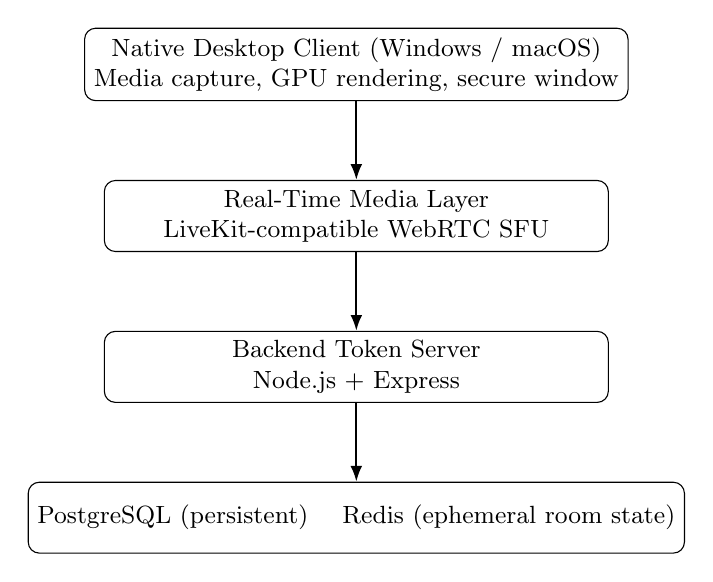
\begin{tikzpicture}[
  node distance=10mm,
  box/.style={draw, rounded corners, minimum width=6.4cm, minimum height=0.9cm, align=center, font=\small},
  arr/.style={-{Latex[length=2mm]}, thick}
]
\node[box] (client) {Native Desktop Client (Windows / macOS)\\Media capture, GPU rendering, secure window};
\node[box, below=of client] (media) {Real-Time Media Layer\\LiveKit-compatible WebRTC SFU};
\node[box, below=of media] (backend) {Backend Token Server\\Node.js + Express};
\node[box, below=of backend, minimum width=6.4cm] (data) {PostgreSQL (persistent) \quad Redis (ephemeral room state)};
\draw[arr] (client) -- (media);
\draw[arr] (media) -- (backend);
\draw[arr] (backend) -- (data);
\end{tikzpicture}
\caption{KioMeet layered system architecture}
\label{fig:architecture}
\end{figure}

\rsection{1.3}{PROBLEM STATEMENT}
The problem addressed by KioMeet is to design and build a native,
cross-platform (Windows and macOS) video conferencing platform that supports
both standard team calls and technical interviews, in which an interviewer's
private material is provably isolated from the shared video stream, while
delivering reliable multi-participant audio/video, screen sharing, recording,
scheduling, and moderation through a secure, tier-gated backend -- without the
overhead and capability limits of browser- or Electron-based solutions.

Figure~\ref{fig:dfd} presents a context-level data-flow diagram (DFD) of the
problem. It shows the external entities that interact with the KioMeet system
and the principal data flows between them, scoping the boundary of the module
undertaken during the internship.

\begin{figure}[h]
\centering
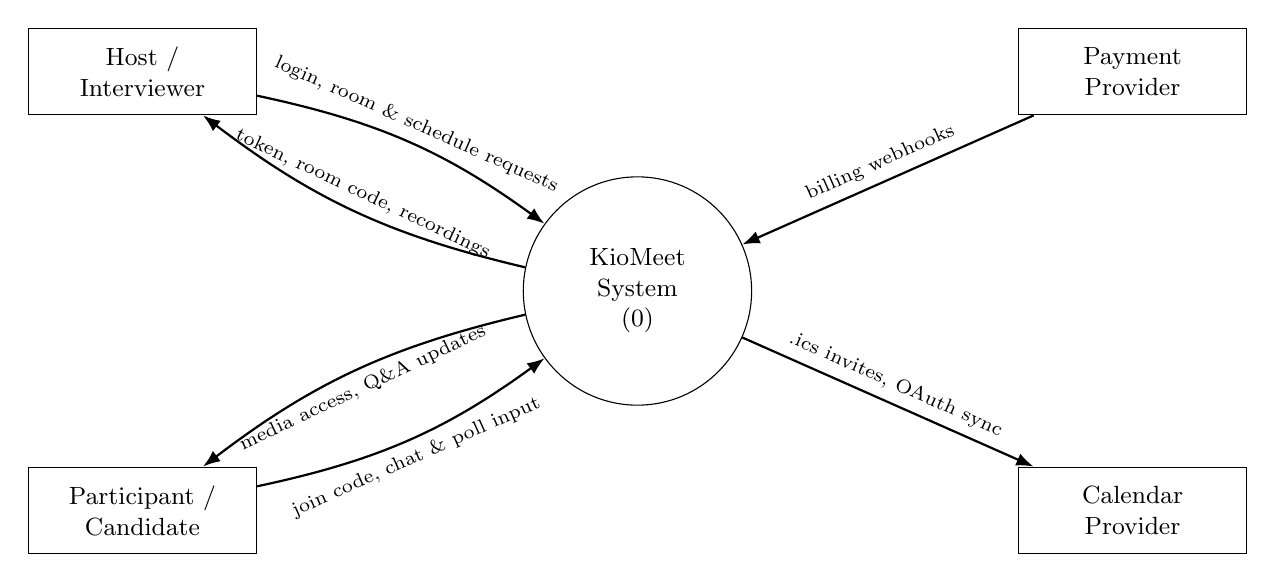
\begin{tikzpicture}[
  entity/.style={draw, minimum width=2.9cm, minimum height=1.1cm, align=center},
  process/.style={draw, circle, minimum size=2.9cm, align=center},
  flow/.style={-{Latex[length=2.2mm]}, thick},
  font=\small
]
\node[process] (sys) {KioMeet\\System\\(0)};
\node[entity] (host) [above left=1.2cm and 3.8cm of sys] {Host /\\Interviewer};
\node[entity] (part) [below left=1.2cm and 3.8cm of sys] {Participant /\\Candidate};
\node[entity] (pay)  [above right=1.2cm and 3.8cm of sys] {Payment\\Provider};
\node[entity] (cal)  [below right=1.2cm and 3.8cm of sys] {Calendar\\Provider};

\draw[flow] (host) to[bend left=12]
  node[sloped,above,font=\scriptsize]{login, room \& schedule requests} (sys);
\draw[flow] (sys) to[bend left=12]
  node[sloped,above,font=\scriptsize]{token, room code, recordings} (host);
\draw[flow] (part) to[bend right=12]
  node[sloped,below,font=\scriptsize]{join code, chat \& poll input} (sys);
\draw[flow] (sys) to[bend right=12]
  node[sloped,below,font=\scriptsize]{media access, Q\&A updates} (part);
\draw[flow] (pay) to
  node[sloped,above,font=\scriptsize]{billing webhooks} (sys);
\draw[flow] (sys) to
  node[sloped,above,font=\scriptsize]{.ics invites, OAuth sync} (cal);
\end{tikzpicture}
\caption{Context-level data-flow diagram (DFD) of the KioMeet system}
\label{fig:dfd}
\end{figure}

\rsection{1.4}{INTERNSHIP ROLE AND SCOPE OF WORK}
Under the Full Stack Development track and the guidance of the PMO, the
scope of work carried out during the internship (12 June -- 7 August 2026)
included:
\begin{itemize}
  \item Contributing to the Node.js/Express backend (\texttt{token-server/}):
        authentication, scheduling, teams, and tier/billing modules.
  \item Building the backend session logic behind KioMeet's secure interview
        mode -- creating and permission-gating a locked \texttt{secure-interview}
        session type that the client uses to restrict the shared view to a
        single designated window.
  \item Implementing the real-time signalling (WebSocket channels) that
        delivers in-call chat messages, live poll results, and Q\&A updates
        to every participant instantly.
  \item Working with PostgreSQL schema migrations and Redis-backed ephemeral
        room state.
  \item Assisting with the \texttt{launch-web} marketing site's waitlist API
        and admin panel.
  \item Participating in weekly PMO evaluation sprints and community code
        reviews.
\end{itemize}

\rsection{1.5}{GOAL AND VISION}
The goal of the internship was twofold: to deliver a working, tested
contribution to KioMeet's backend within the eight-week engagement, and to
build practical competence in authentication design, relational data
modelling, and real-time systems -- skills directly transferable to
production full-stack engineering roles.

\rsection{1.6}{REPORT OUTLINE}
The remainder of this report is organised as follows. Chapter 2 specifies the
requirements of the module undertaken. Chapter 3 presents the system design.
Chapter 4 describes the testing approach and results. Chapter 5 discusses the
outcomes achieved during the internship. Chapter 6 concludes the report and
outlines scope for future work.

% ---------------------------------------------------------------------
\rchapter{REQUIREMENT SPECIFICATION}

This chapter specifies the functional and non-functional requirements of the
KioMeet backend module undertaken during the internship.

\rsection{2.1}{USER CHARACTERISTICS}
KioMeet serves two primary user classes relevant to the backend module:
\begin{itemize}
  \item \textbf{Hosts / Interviewers} -- create rooms, schedule meetings,
        manage recordings, and moderate participants.
  \item \textbf{Participants / Candidates} -- join rooms via a 6-character
        code, respond to lobby/password gates, and participate in chat,
        polls, and Q\&A.
\end{itemize}
Both classes authenticate via the JWT-based auth flow, and their accessible
features are gated by subscription tier (free, pro, hiring).

\rsection{2.2}{USE CASES (FUNCTIONAL REQUIREMENTS)}
Table~\ref{tab:usecases} summarises the principal use cases implemented or
touched during the internship.

\begin{table}[h]
\centering
\caption{Principal use cases of the backend module}
\label{tab:usecases}
\begin{tabular}{@{}p{3.2cm}p{9.5cm}@{}}
\toprule
Use Case & Description \\
\midrule
Register / Login & User registers or logs in; receives a short-lived JWT access token and a rotating refresh token. \\
Refresh Session & Client exchanges a valid refresh token for a new access token; tier is re-read from the database on every refresh. \\
Create Room & Host creates a call or interview room; a 6-character join code is generated with a 24-hour expiry in Redis. \\
Join Room & Participant joins via room code, optional password, and lobby approval. \\
Schedule Meeting & Host schedules a meeting with invitees, who receive an \texttt{.ics} email invite; synced to Apple/Google/Outlook calendars. \\
Manage Team & Team owner/admin invites members, assigns roles, and manages team membership. \\
Start Secure Interview & Host starts a locked \texttt{secure-interview} session; the backend restricts the session to a single shared-window grant that the client enforces on screen. \\
Live Chat / Poll / Q\&A & Backend relays chat messages, poll launches/results, and Q\&A items over a per-room WebSocket channel so every participant updates in real time. \\
Enforce Tier Limits & Backend enforces per-tier limits on recording mode, poll count, and room capacity. \\
\bottomrule
\end{tabular}
\end{table}

\rsubsection{2.2.1}{Use Case Diagram}
A simplified use-case view of the authentication and room-management flow is
as follows: an \textit{Actor (Host/Participant)} interacts with
\textit{Register/Login}, \textit{Create or Join Room}, and \textit{Schedule
Meeting}, each of which depends on the \textit{Authenticate} use case for
authorization.

\rsection{2.3}{DEPENDENCIES}
The module depends on: Node.js 20+, Express, PostgreSQL 15+, Redis 7+, a
LiveKit-compatible WebRTC server, and third-party calendar OAuth providers
(Google, Microsoft/Outlook).

\rsection{2.4}{PERFORMANCE REQUIREMENTS}
\begin{itemize}
  \item Access tokens must expire within 15 minutes; this bounds the
        maximum staleness of a user's tier after a billing change.
  \item Room lookups and join-code validation must complete within Redis's
        typical sub-millisecond read latency to avoid perceptible join delay.
  \item The system must support rooms of up to 50 participants without
        degrading signalling responsiveness.
\end{itemize}

\rsection{2.5}{HARDWARE REQUIREMENTS}
\begin{itemize}
  \item Development: a standard laptop/desktop capable of running Node.js,
        PostgreSQL, and Redis locally (minimum 8\,GB RAM recommended).
  \item Deployment: a server or cloud instance able to host the Express
        backend, PostgreSQL, and Redis, reachable by the LiveKit WebRTC
        server and the native desktop clients.
\end{itemize}

\rsection{2.6}{CONSTRAINTS AND ASSUMPTIONS}
\begin{itemize}
  \item All financial/tier state is authoritative only in \texttt{users.tier}
        in PostgreSQL; the client is never trusted to assert its own tier.
  \item The internship module could be developed and demonstrated against a
        local PostgreSQL/Redis instance; access to the production LiveKit
        deployment was out of scope for the internship.
  \item Development followed the engagement's confidentiality terms (Offer
        Ref.\ IWP-STU-2026-0904): internal implementation detail beyond what
        is already documented in the project's public-facing materials is
        presented here only at a level suitable for an academic report.
\end{itemize}

% ---------------------------------------------------------------------
\rchapter{SYSTEM DESIGN}

\rsection{3.1}{ARCHITECTURE}
The backend follows a layered Express architecture with a clear separation of
concerns: \texttt{auth.js} handles login, logout, and token issuance;
\texttt{billing.js} handles subscription and tier state; \texttt{scheduling.js}
and \texttt{calendar.js} handle meeting scheduling and OAuth calendar sync;
\texttt{teams.js} handles team management; and a shared \texttt{middleware}
layer (\texttt{requireAuth}, \texttt{requireTier}) reads state and makes no
business decisions of its own.

\rsubsection{3.1.1}{Authentication Design}
A two-token model is used: a short-lived (15-minute) JWT access token signed
with HS256, and a long-lived (30-day) opaque refresh token stored only as a
SHA-256 hash in the database. Refresh requests are processed inside an atomic
transaction with family-based theft detection: if a revoked token is
re-presented, the entire token family is revoked and the session is forced to
re-authenticate.

\rsubsection{3.1.2}{Tier and Billing Design}
Subscription tier changes follow an explicit state machine
(\texttt{none} $\rightarrow$ \texttt{trialing}/\texttt{active}
$\rightarrow$ \texttt{past\_due}/\texttt{canceled}, with recovery and
chargeback paths) and are driven exclusively by signed payment-provider
webhooks, never by client input. All tier changes are atomic and
accompanied by an append-only audit record in \texttt{user\_tier\_history}.

\rsubsection{3.1.3}{Secure Interview Session Design}
A room may be started in a locked \texttt{secure-interview} mode. On session
start, the backend issues the host a single \textit{share grant} scoped to
one window handle; the client enforces the actual window-level capture
restriction, but it is the backend that creates the session record, marks it
\texttt{locked}, and rejects any attempt (by either participant) to attach a
second shared surface to that session. This keeps the isolation guarantee
backend-verifiable rather than resting purely on client-side behaviour.

\rsubsection{3.1.4}{Real-Time Signalling}
Chat, polls, and Q\&A are delivered over a per-room WebSocket channel
(separate from the WebRTC media path). Each event (a new chat message, a poll
being launched, a vote being cast, a question being asked or marked answered)
is validated against the sender's role and tier, persisted, and then
broadcast to every connected participant in that room, so the host and all
participants see the same state update within the same round trip.

\rsection{3.2}{DATABASE DESIGN}
Persistent entities (\texttt{users}, \texttt{meetings},
\texttt{meeting\_participants}, \texttt{recording\_sessions},
\texttt{scheduled\_meetings}, \texttt{meeting\_invitees}, \texttt{teams},
\texttt{team\_members}) are modelled in PostgreSQL with explicit foreign-key
relationships and a deliberate \texttt{ON DELETE} policy per relationship
(e.g.\ \texttt{RESTRICT} on purchase history, \texttt{CASCADE} on refresh
tokens). Migrations are forward-only, numbered sequentially, and tracked in a
\texttt{schema\_migrations} table so re-running the migration runner is safe
and idempotent. Ephemeral room state (active room codes, presence) is kept in
Redis with a 24-hour TTL rather than in PostgreSQL, since it does not need to
survive beyond a room's lifetime.

\rsection{3.3}{API DESIGN}
Every endpoint follows a consistent error contract --
\texttt{\{ error, code, requestId \}} -- so the client can switch on a stable
machine-readable \texttt{code} (e.g.\ \texttt{TOKEN\_EXPIRED},
\texttt{TIER\_INSUFFICIENT}, \texttt{RATE\_LIMITED}) rather than parsing
human-readable text. Security headers (HSTS, \texttt{Cache-Control: no-store},
\texttt{X-Content-Type-Options}) are applied globally via middleware, and
sensitive fields (\texttt{password}, \texttt{refreshToken}) are scrubbed
before any logging.

\rsection{3.4}{GUI / INTERFACE DESIGN}
On the client side, the relevant interfaces for the module worked on are the
connection setup panel (server URL, room code entry), the schedule panel
(meeting creation and invitee management), and the recording list panel. On
the web side, the \texttt{launch-web} marketing site exposes a public
waitlist form and a password-protected admin panel for reviewing signups,
both served from the same Express process as static assets plus a JSON API.

\rsection{3.5}{PACKAGE / MODULE HIERARCHY}
The backend (\texttt{token-server/}) is organised as a flat set of
single-responsibility Express routers/modules
(\texttt{auth, billing, scheduling, calendar, teams, mailer, crypto,
migrate}) wired together in \texttt{index.js}, which also mounts the health
check endpoint and global security middleware.

% ---------------------------------------------------------------------
\rchapter{TESTING}

\rsection{4.1}{TEST PLAN}
Testing of the module followed the project's existing conventions: unit tests
for isolated logic (token signing/verification, tier-transition validation,
webhook-signature checks) and integration tests against a local PostgreSQL
and Redis instance for end-to-end flows (register $\rightarrow$ login
$\rightarrow$ refresh $\rightarrow$ create room $\rightarrow$ join room).
Where a live dependency (e.g.\ the production LiveKit server) was
unreachable, tests were designed to skip gracefully rather than fail,
consistent with the project's existing \texttt{XCTSkip}-style pattern on the
native client test suite.

\rsection{4.2}{TEST REPORT}
\begin{itemize}
  \item Authentication flow -- verified correct issuance and rejection of
        expired vs.\ invalid access tokens, and family-wide revocation on
        reuse of a revoked refresh token.
  \item Tier enforcement -- verified that \texttt{requireTier} middleware
        fails closed (403 \texttt{TIER\_INSUFFICIENT}) when a user's tier is
        \texttt{null} or below the required rank.
  \item Scheduling -- verified that an \texttt{.ics} invite is generated for
        each invitee and that a scheduled meeting appears correctly under
        both the host's and the invitee's upcoming-meetings list.
  \item Webhook idempotency -- verified that replaying the same billing
        webhook event id a second time is a no-op (\texttt{already\_processed})
        and does not duplicate a tier change.
  \item Secure interview sessions -- verified that a second share-grant
        request against an already-locked session is rejected, and that the
        session record correctly reflects \texttt{locked} state for the
        duration of the interview.
  \item Real-time signalling -- verified that a chat message, poll result, or
        Q\&A update sent by one participant is broadcast to and received by
        every other connected participant in the same room.
\end{itemize}

\rsection{4.3}{DEFECT LOG}
Representative issues identified and resolved during the internship period
included an edge case where a webhook received before its corresponding user
record existed was silently dropped (fixed by queuing and retrying), and a
missing \texttt{Retry-After} header on one rate-limited endpoint (fixed to
match the project's documented error contract).

\rsection{4.4}{INSTALLATION AND END-USER INSTRUCTIONS}
The backend is run locally via \texttt{npm install} followed by
\texttt{node migrate.js} (to apply schema migrations) and \texttt{node
index.js} (or \texttt{npx nodemon index.js} for development), after
configuring \texttt{token-server/.env} per \texttt{.env.example}. A healthy
instance responds to \texttt{GET /health} with Redis and PostgreSQL
connection status.

% ---------------------------------------------------------------------
\rchapter{RESULTS AND DISCUSSION}

\rsection{5.1}{OUTCOMES ACHIEVED}
By the end of the internship, the assigned backend contributions were
functional, tested against a local PostgreSQL/Redis environment, and
reviewed by the PMO. Table~\ref{tab:progress} summarises the weekly progress
over the eight-week engagement.

\begin{table}[h]
\centering
\caption{Weekly progress during the internship}
\label{tab:progress}
\begin{tabular}{@{}p{1.4cm}p{3.0cm}p{9.0cm}@{}}
\toprule
Week & Dates (2026) & Summary of Work \\
\midrule
1 & 12 -- 18 Jun & Onboarding, codebase walkthrough, environment setup (Node.js, PostgreSQL, Redis). \\
2 & 19 -- 25 Jun & Studied authentication module; implemented unit tests for JWT issuance/verification. \\
3 & 26 Jun -- 2 Jul & Worked on refresh-token rotation and family-based theft detection. \\
4 & 3 -- 9 Jul & Contributed to scheduling module (\texttt{.ics} invites, calendar sync touchpoints). \\
5 & 10 -- 16 Jul & Implemented and tested tier-enforcement middleware edge cases. \\
6 & 17 -- 23 Jul & Worked on team management module (role-based permissions); built the secure-interview session/locking logic. \\
7 & 24 -- 30 Jul & Implemented real-time chat/poll/Q\&A signalling; integration testing across auth, scheduling, teams, and signalling modules. \\
8 & 31 Jul -- 7 Aug & Bug fixes, documentation, final PMO review and demo. \\
\bottomrule
\end{tabular}
\end{table}

\rsection{5.2}{DISCUSSION}
The internship provided direct exposure to production-oriented backend
patterns that are often only discussed abstractly in coursework: atomic
multi-step database transactions, fail-closed authorization, idempotent
webhook processing, and a consistent machine-readable API error contract.
Working within an existing, opinionated codebase (rather than a greenfield
project) also required adapting to established conventions -- for instance,
the project's strict separation between \texttt{auth.js} and
\texttt{billing.js} -- which reinforced the practical value of separation of
concerns beyond its theoretical treatment in software engineering courses.

\rsection{5.3}{SKILLS GAINED}
\begin{itemize}
  \item Practical experience with Node.js/Express, PostgreSQL, and Redis in
        a real backend.
  \item JWT-based authentication design, including refresh-token rotation
        and theft detection.
  \item Writing and reasoning about idempotent, webhook-driven business
        logic.
  \item Designing backend-verifiable session state for a security-sensitive
        feature (secure interview mode), rather than relying solely on
        client-side enforcement.
  \item Building real-time, WebSocket-based features (chat, polls, Q\&A) and
        reasoning about event ordering and broadcast correctness.
  \item Collaborative, review-driven development under a PMO-style
        supervision model with weekly evaluation.
\end{itemize}

% ---------------------------------------------------------------------
\rchapter{CONCLUSION AND FUTURE SCOPE}

This eight-week internship at IndiWebPros, under the Full Stack Development
track, provided practical, supervised experience contributing to KioMeet, a
real cross-platform video conferencing and secure technical-interview
platform. The engagement covered the full backend lifecycle relevant to the
module undertaken -- requirement understanding, design, implementation, and
testing -- and resulted in a working, reviewed contribution to the
authentication, scheduling, team-management, secure-interview-session, and
real-time signalling modules of the product.

\rsection{6.1}{FUTURE SCOPE}
Future enhancements identified but out of scope for the internship period
include: extending multi-track cloud recording to additional storage
backends beyond S3, adding row-level security policies to more user-owned
tables, and building automated end-to-end tests that exercise the full
client-to-backend flow against a live LiveKit instance rather than mocked
media tracks.

% =====================================================================
%  REFERENCES
% =====================================================================
\rchapterstar{REFERENCES}
\begin{thebibliography}{9}
  \bibitem{webrtc} WebRTC --- Official Project Documentation. \url{https://webrtc.org}
  \bibitem{livekit} LiveKit --- Open-Source WebRTC SFU Documentation. \url{https://docs.livekit.io}
  \bibitem{jwt} IETF RFC 7519 --- JSON Web Token (JWT).
  \bibitem{rfc8825} IETF RFC 8825 --- Overview: Real-Time Protocols for Browser-Based Applications (WebRTC).
  \bibitem{express} Express.js --- Official Documentation. \url{https://expressjs.com}
  \bibitem{postgres} PostgreSQL 15 --- Official Documentation. \url{https://www.postgresql.org/docs/15/}
  \bibitem{redis} Redis --- Official Documentation. \url{https://redis.io/docs/}
  \bibitem{offerletter} IndiWebPros, \textit{Offer of Internship with IndiWebPros}, Ref.\ IWP-STU-2026-0904, 07 June 2026 (internal document).
\end{thebibliography}

% =====================================================================
%  APPENDICES
% =====================================================================
\rchapterstar{APPENDIX I}
\noindent
Sample backend health-check response (\texttt{GET /health}):
\begin{verbatim}
{
  "status": "ok",
  "redis": "connected",
  "postgres": "connected"
}
\end{verbatim}

\rchapterstar{APPENDIX II: LIST OF SOFT OUTPUTS}
\begin{enumerate}
  \item Soft copy (PDF) of this report.
  \item Offer-of-internship letter from IndiWebPros (Ref.\ IWP-STU-2026-0904).
  \item Relevant source-code modules contributed to during the internship.
  \item Weekly progress notes corresponding to Table~\ref{tab:progress}.
\end{enumerate}

\end{document}
